\documentclass[11pt]{article}

\usepackage[margin=1in]{geometry}
\usepackage{amsmath, amssymb}
\usepackage{tikz}
\usetikzlibrary{arrows.meta, positioning, fit, backgrounds, calc}
\usepackage{float}
\usepackage{tcolorbox}
\tcbuselibrary{skins, breakable}
\usepackage{xcolor}
\usepackage{enumitem}
\usepackage{hyperref}
\hypersetup{colorlinks=true, linkcolor=blue!55!black, urlcolor=blue!55!black}

\definecolor{accent}{RGB}{30,90,160}
\definecolor{accent2}{RGB}{170,60,30}
\definecolor{soft}{RGB}{238,243,250}
\definecolor{soft2}{RGB}{250,243,236}

\newtcolorbox{keybox}[1]{
  colback=soft, colframe=accent, fonttitle=\bfseries,
  title=#1, breakable, boxrule=0.6pt, arc=2pt, left=6pt, right=6pt}

\newtcolorbox{watchbox}[1]{
  colback=soft2, colframe=accent2, fonttitle=\bfseries,
  title=#1, breakable, boxrule=0.6pt, arc=2pt, left=6pt, right=6pt}

\title{\textbf{Mann \S3.1.2 --- Representations}\\[2pt]
\large A Plain--Language Walkthrough (with diagrams)}
\author{Reading companion --- Mann, \emph{An Introduction to Particle Physics
and the Standard Model}, Ch.~3}
\date{2026--05--18}

\begin{document}
\maketitle

\noindent\textbf{Where we are.} In \S3.1.1 we learned that a \emph{symmetry}
is described by a \emph{group}: a set of transformations that is closed, has an
identity, has inverses, and is associative. That was abstract --- just symbols
$g_i$ and a rule ``$\bullet$''. Section 3.1.2 answers the practical question:
\emph{what do these transformations actually act on, and how do we compute with
them?} The answer is \textbf{matrices}, and the bridge is the idea of a
\textbf{representation}.

\bigskip
\hrule
\bigskip

\section*{1. What does a symmetry transformation act \emph{on}?}

In particle physics, the object that gets transformed by a symmetry is almost
always the \textbf{wavefunction} of a particle (or set of particles). Mann
points out that, unlike intro QM where the wavefunction is a single complex
function, here it is generally a \textbf{multi--component complex column
vector} living in some abstract space. A symmetry operation acts on it by
\textbf{matrix multiplication}.

\begin{figure}[H]
\centering
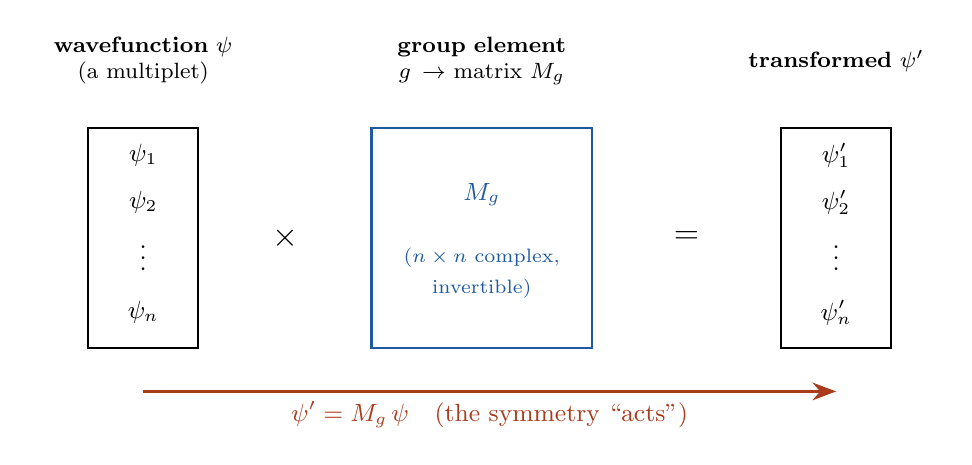
\begin{tikzpicture}[every node/.style={font=\small}]
  % column vector psi
  \draw[thick] (-4.0,-1.4) rectangle (-2.6,1.4);
  \node at (-3.3,1.05) {$\psi_1$};
  \node at (-3.3,0.45) {$\psi_2$};
  \node at (-3.3,-0.15) {$\vdots$};
  \node at (-3.3,-0.95) {$\psi_n$};
  \node[font=\footnotesize, align=center, text width=2.7cm]
       at (-3.3,2.25) {\textbf{wavefunction} $\psi$\\(a multiplet)};

  % matrix M_g
  \draw[thick, accent] (-0.4,-1.4) rectangle (2.4,1.4);
  \node[accent] at (1.0,0.55) {$M_g$};
  \node[accent, font=\scriptsize] at (1.0,-0.25) {($n\times n$ complex,};
  \node[accent, font=\scriptsize] at (1.0,-0.65) {invertible)};
  \node[font=\footnotesize, align=center, text width=3.0cm]
       at (1.0,2.25) {\textbf{group element} $g\to$ matrix $M_g$};

  % result
  \draw[thick] (4.8,-1.4) rectangle (6.2,1.4);
  \node at (5.5,1.05) {$\psi_1'$};
  \node at (5.5,0.45) {$\psi_2'$};
  \node at (5.5,-0.15) {$\vdots$};
  \node at (5.5,-0.95) {$\psi_n'$};
  \node[font=\footnotesize, align=center, text width=2.5cm]
       at (5.5,2.25) {\textbf{transformed} $\psi'$};

  % operators
  \node at (-1.5,0) {\large $\times$};
  \node at (3.6,0) {\large $=$};
  \draw[-{Stealth[length=3mm]}, accent2, thick] (-3.3,-1.95) -- (5.5,-1.95)
        node[midway, below, accent2, font=\small]
        {$\psi' = M_g\,\psi$ \ \ (the symmetry ``acts'')};
\end{tikzpicture}
\caption{A symmetry transformation $g$ is realized as an $n\times n$ complex
matrix $M_g$ that multiplies the wavefunction column vector $\psi$ and
``rotates'' it into a new one $\psi'$. The number of components $n$ is the
\emph{dimension} of the representation.}
\end{figure}

\noindent\textbf{Reading the figure.} The left box is the particle's
wavefunction written as a stack of complex numbers (a \emph{multiplet}). The
middle box is the abstract group element $g$ \emph{turned into} a concrete
matrix $M_g$. Multiplying gives a new wavefunction $\psi'$. Crucially, the
matrix must be \emph{square and invertible} --- those requirements are forced
on us by the group axioms, as we will see.

\section*{2. The core idea: a representation is a ``translation dictionary''}

A group is abstract; matrices are concrete and computable. A
\textbf{representation} is a rule that assigns a matrix $M_g$ to every group
element $g$ \emph{in a way that respects the group's multiplication table}:

\begin{keybox}{Definition (in words and symbols)}
For every $g\in G$ there is a matrix $M_g$ such that
\[
g_1\bullet g_2 = g_3 \quad\Longrightarrow\quad M_{g_1} M_{g_2} = M_{g_3}.
\]
``Combine first, then translate'' gives the \emph{same} answer as ``translate
first, then multiply the matrices.'' Such a structure--preserving map
$\rho: G \to \{M_g\}$ is called a \textbf{representation} (mathematically, a
\emph{homomorphism}). A $d$--dimensional representation uses $d\times d$
matrices.
\end{keybox}

\begin{figure}[H]
\centering
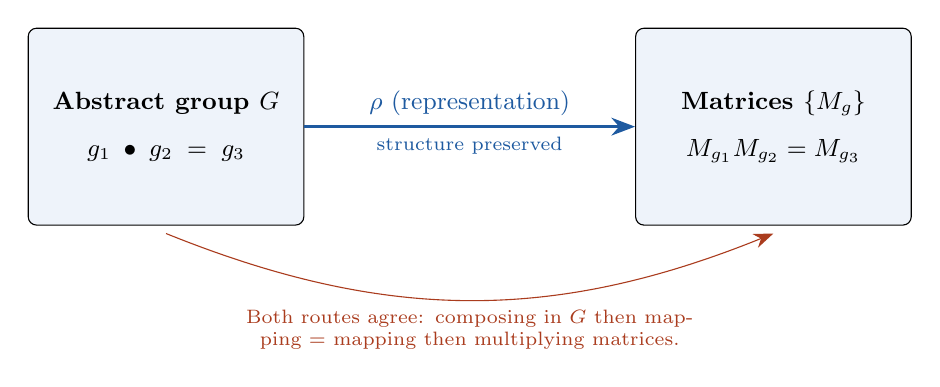
\begin{tikzpicture}[every node/.style={font=\small},
   box/.style={draw, rounded corners=3pt, minimum width=3.5cm,
               minimum height=2.5cm, align=center}]
  \node[box, fill=soft] (G) {\textbf{Abstract group }$G$\\[6pt]
        $g_1 \;\bullet\; g_2 \;=\; g_3$};
  \node[box, fill=soft, right=4.2cm of G] (M)
       {\textbf{Matrices }$\{M_g\}$\\[6pt]
        $M_{g_1} M_{g_2} = M_{g_3}$};

  \draw[-{Stealth[length=3mm]}, accent, very thick]
       (G.east) -- node[above]{$\rho$ (representation)}
                   node[below]{\scriptsize structure preserved} (M.west);

  \draw[-{Stealth[length=2.5mm]}, accent2] ($(G.south)+(0,-0.1)$)
       to[bend right=22]
       node[below, font=\scriptsize, text width=7.5cm, align=center]
       {Both routes agree: composing in $G$ then mapping
        $=$ mapping then multiplying matrices.}
       ($(M.south)+(0,-0.1)$);
\end{tikzpicture}
\caption{A representation $\rho$ is a ``dictionary'' from abstract group
elements to matrices that keeps the multiplication table intact. This is the
single most important sentence in \S3.1.2.}
\end{figure}

\noindent\textbf{Why this is powerful.} Once the dictionary exists, every
abstract symmetry question becomes ordinary (if tedious) \textbf{matrix
algebra} --- something we can actually compute.

\section*{3. Why matrices are the perfect choice}

Mann notes three ``freebies'' you get automatically by using matrices:

\begin{itemize}[leftmargin=1.4em, itemsep=2pt]
  \item \textbf{Associativity is automatic} --- matrix multiplication is
        associative, so that group axiom is satisfied for free.
  \item \textbf{Inverses force invertibility} --- the group's inverse axiom
        means every $M_g$ must be an \emph{invertible} matrix. This sharply
        restricts which matrices can appear.
  \item \textbf{Identity is trivial} --- the group identity $I$ is just the
        identity matrix $\mathbb{1}$.
\end{itemize}

\section*{4. Three things that surprise people}

\begin{figure}[H]
\centering
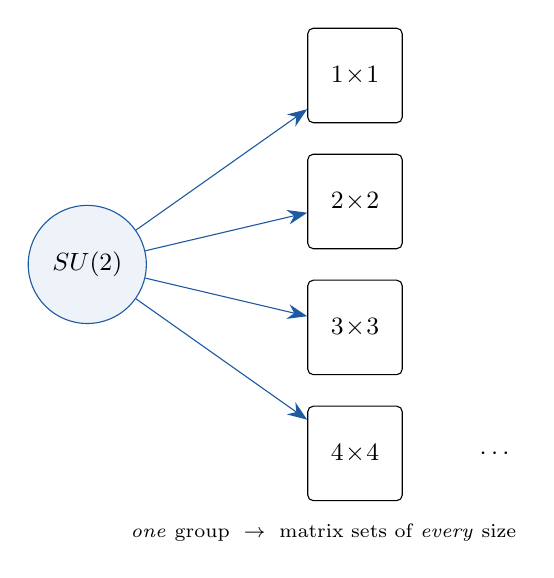
\begin{tikzpicture}[every node/.style={font=\small},
  grp/.style={circle, draw=accent, fill=soft, minimum size=1.5cm},
  mat/.style={draw, rounded corners=2pt, fill=white, minimum width=1.2cm,
              minimum height=1.2cm}]

  \node[grp] (su2) at (0,0) {$SU(2)$};
  \node[mat] (m1) at (3.4, 2.4) {$1\!\times\!1$};
  \node[mat] (m2) at (3.4, 0.8) {$2\!\times\!2$};
  \node[mat] (m3) at (3.4,-0.8) {$3\!\times\!3$};
  \node[mat] (m4) at (3.4,-2.4) {$4\!\times\!4$};
  \node at (5.2,-2.4) {$\cdots$};

  \foreach \m in {m1,m2,m3,m4}
     \draw[-{Stealth[length=2.5mm]}, accent] (su2) -- (\m);
  \node[align=center, font=\scriptsize] at (3.0,-3.4)
       {\emph{one} group $\;\to\;$ matrix sets of \emph{every} size};
\end{tikzpicture}
\caption{(a) \textbf{Representations are not unique.} The very same group ---
here $SU(2)$ --- can be represented by matrices of dimension
$1,2,3,4,\dots$ A group has \emph{infinitely many} representations.}
\end{figure}

\begin{figure}[H]
\centering
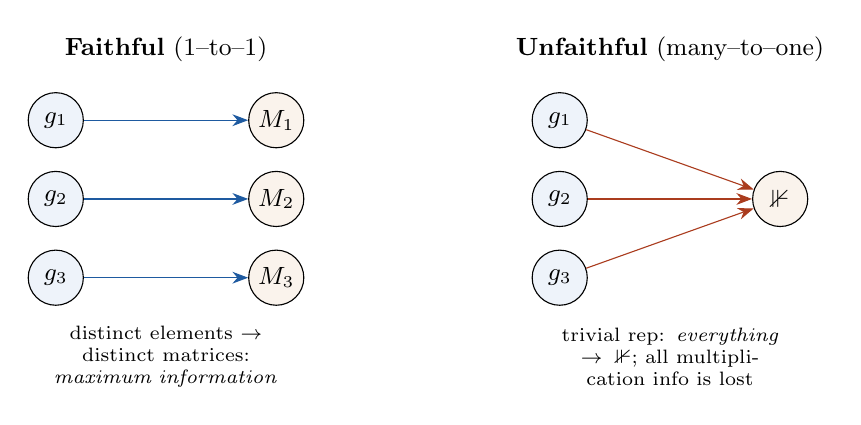
\begin{tikzpicture}[every node/.style={font=\small},
   g/.style={circle, draw, fill=soft, minimum size=0.7cm, inner sep=0pt},
   mm/.style={circle, draw, fill=soft2, minimum size=0.7cm, inner sep=0pt}]

  % Faithful: bijection
  \node at (-3.4,2.4) {\textbf{Faithful} (1--to--1)};
  \node[g] (a1) at (-4.8,1.5) {$g_1$};
  \node[g] (a2) at (-4.8,0.5) {$g_2$};
  \node[g] (a3) at (-4.8,-0.5) {$g_3$};
  \node[mm] (b1) at (-2.0,1.5) {$M_1$};
  \node[mm] (b2) at (-2.0,0.5) {$M_2$};
  \node[mm] (b3) at (-2.0,-0.5) {$M_3$};
  \draw[-{Stealth[length=2mm]}, accent] (a1)--(b1);
  \draw[-{Stealth[length=2mm]}, accent] (a2)--(b2);
  \draw[-{Stealth[length=2mm]}, accent] (a3)--(b3);
  \node[font=\scriptsize, text width=3.2cm, align=center] at (-3.4,-1.5)
       {distinct elements $\to$ distinct matrices: \emph{maximum information}};

  % Unfaithful: many-to-one (trivial rep)
  \node at (3.0,2.4) {\textbf{Unfaithful} (many--to--one)};
  \node[g] (c1) at (1.6,1.5) {$g_1$};
  \node[g] (c2) at (1.6,0.5) {$g_2$};
  \node[g] (c3) at (1.6,-0.5) {$g_3$};
  \node[mm] (d1) at (4.4,0.5) {$\mathbb{1}$};
  \draw[-{Stealth[length=2mm]}, accent2] (c1)--(d1);
  \draw[-{Stealth[length=2mm]}, accent2] (c2)--(d1);
  \draw[-{Stealth[length=2mm]}, accent2] (c3)--(d1);
  \node[font=\scriptsize, text width=3.4cm, align=center] at (3.0,-1.5)
       {trivial rep: \emph{everything} $\to \mathbb{1}$; all multiplication
        info is lost};
\end{tikzpicture}
\caption{(b) \textbf{Representations need not be faithful.} If the map is
1--to--1 (left), the representation is \emph{faithful} and carries the maximum
information about the group. Often several elements share one matrix (right);
the extreme case maps \emph{everything} to the identity.}
\end{figure}

\noindent And the third point:
\begin{itemize}[leftmargin=1.4em, itemsep=2pt]
  \item \textbf{The fundamental representation.} If the group already
        \emph{is} a set of matrices, that set is automatically a faithful
        representation of itself --- called the \textbf{fundamental
        representation}. (Example: $SU(2)$ as $2\times2$ unitary matrices is
        its own fundamental rep, but it \emph{also} has the $1,3,4,\dots$
        dimensional reps from Fig.~3a.)
\end{itemize}

\section*{5. Why ever use an \emph{unfaithful} representation?}

It seems wasteful to throw away information --- so why bother? Mann's footnote
gives the key example: map every group element to $\pm\mathbb{1}$. You lose
almost everything, but you \emph{keep} one crucial bit: the even/odd character
of each element. For the rotation group this single bit tells you whether a
transformation is a \textbf{reflection}, i.e.\ whether it has \textbf{odd
parity} --- already real physics. Lesson: use the smallest representation that
still carries the information you actually need.

\begin{watchbox}{Common confusions to avoid}
\begin{itemize}[leftmargin=1.2em, itemsep=2pt]
  \item ``Representation = the group.'' \textbf{No} --- it is one \emph{matrix
        picture} of the group; there are infinitely many.
  \item ``Bigger matrices = more fundamental.'' \textbf{No} --- the
        \emph{fundamental} rep is the group's own defining matrices; larger
        reps are derived.
  \item ``Unfaithful reps are useless.'' \textbf{No} --- they isolate a
        specific feature (e.g.\ parity) cleanly.
  \item Dimension of the rep $=$ number of wavefunction components $=$ size of
        the multiplet (doublet, triplet, $\dots$).
\end{itemize}
\end{watchbox}

\begin{keybox}{One--paragraph takeaway}
A \textbf{representation} turns the abstract group of a symmetry into concrete
$d\times d$ invertible complex matrices that act on a particle's wavefunction
multiplet, \emph{preserving the group's multiplication table}. The matrix
viewpoint makes associativity, inverses, and the identity automatic and lets
you actually \emph{calculate}. A group has infinitely many representations of
many dimensions; they may be \emph{faithful} (1--to--1, maximal information)
or not; the group's own defining matrices form the \emph{fundamental}
representation. Choosing a representation is choosing how much of the
symmetry's information you want to keep for the physics at hand --- which sets
up the next section's question: what are the \emph{irreducible} (non-redundant)
representations?
\end{keybox}

\end{document}
